% -*- mode: LaTeX; TeX-PDF-mode: t; -*- 
% LaTeX path to the root directory of the current project
% from the directory in which this file resides
% and path to econtexPaths which defines the rest of the paths like \FigDir
\providecommand{\econtexRoot}{}\renewcommand{\econtexRoot}{.}
\providecommand{\econtexPaths}{}\renewcommand{\econtexPaths}{econtexPaths}
% -*- mode: LaTeX; TeX-PDF-mode: t; -*- 
% The \commands below are required to allow sharing of the same base code via Github between TeXLive on a local machine and Overleaf (which is a proxy for "a standard distribution of LaTeX").  This is an ugly solution to the requirement that custom LaTeX packages be accessible, and that Overleaf prohibits symbolic links
\providecommand{\packages}{\econtexRoot/Resources/texmf-local/tex/latex}
\providecommand{\econtex}{\packages/econtex}
\providecommand{\econark}{\econtexRoot/Resources/texmf-local/tex/latex/econark}
\providecommand{\econtexSetup}{\econtexRoot/Resources/texmf-local/tex/latex/econtexSetup}
\providecommand{\econarkSetup}{\econtexRoot/Resources/texmf-local/tex/latex/econarkSetup}
\providecommand{\econtexShortcuts}{\econtexRoot/Resources/texmf-local/tex/latex/econtexShortcuts}
\providecommand{\econtexBibMake}{\econtexRoot/Resources/texmf-local/tex/latex/econtexBibMake}
\providecommand{\econtexBibStyle}{\econtexRoot/Resources/texmf-local/bibtex/bst/econtex}
\providecommand{\econtexBib}{economics}
\providecommand{\notes}{\econtexRoot/Resources/texmf-local/tex/latex/handout}
\providecommand{\handoutSetup}{\econtexRoot/Resources/texmf-local/tex/latex/handoutSetup}
\providecommand{\handoutShortcuts}{\econtexRoot/Resources/texmf-local/tex/latex/handoutShortcuts}
\providecommand{\handoutBibMake}{\econtexRoot/Resources/texmf-local/tex/latex/handoutBibMake}
\providecommand{\handoutBibStyle}{\econtexRoot/Resources/texmf-local/bibtex/bst/handout}

\providecommand{\FigDir}{\econtexRoot/Figures}
\providecommand{\CodeDir}{\econtexRoot/Code}
\providecommand{\DataDir}{\econtexRoot/Data}
\providecommand{\SlideDir}{\econtexRoot/Slides}
\providecommand{\TableDir}{\econtexRoot/Tables}
\providecommand{\ApndxDir}{\econtexRoot/Appendices}

\providecommand{\ResourcesDir}{\econtexRoot/Resources}
\providecommand{\rootFromOut}{..} % APFach back to root directory from output-directory
\providecommand{\LaTeXGenerated}{\econtexRoot/LaTeX} % Put generated files in subdirectory
\providecommand{\econtexPaths}{\econtexRoot/Resources/econtexPaths}
\providecommand{\LaTeXInputs}{\econtexRoot/Resources/LaTeXInputs}
\providecommand{\LtxDir}{LaTeX/}
\providecommand{\EqDir}{\econtexRoot/Equations} % Put generated files in subdirectory

\providecommand{\titlepagecustom}{\LaTeXInputs/titlepagecustom}


\documentclass[\econtexRoot/HAFiscal]{subfiles}
\onlyinsubfile{\externaldocument{\econtexRoot/HAFiscal}} % Get xrefs -- esp to apndx -- from main file; only works if main file has already been compiled

\begin{document}

\addcontentsline{toc}{section}{Appendices} % label the section "Appendices"

\hypertarget{Appendices}{} % Allows link to [url-of-paper]#Appendices
\ifthenelse{\boolean{Web}}{}{% Web version has no page headers
  \chead[Appendices]{Appendices}      % but PDF version does
  \appendixpage % Reset formatting for appendices
} 

\hypertarget{Estimating-discount-factor-distributions-for-different-interest-rates}{}\par\section{Estimating discount factor distributions for different interest rates}
\notinsubfile{\label{app:DF_R}}

Figure~\ref{fig:LorenzPtsrobustnessR} shows the fit of the liquid wealth distribution for interest rates of $0.5$ percent and $1.5$ percent per quarter. In both cases, the estimation exactly matches the median liquid wealth to permanent income ratios for each education group listed in Panel~B of Table~\ref{tab:estimBetas}. 

% \begin{table}{th}
%   \begin{center}
%     \begin{tabular}{lccc}
        %         \multicolumn{4}{l}{Panel (B) Estimation targets} \\ \midrule
        %         & Dropout & Highschool & College \\ \midrule
        %         Median LW/PI (data) & 4.64 & 30.2 & 112.8 \\ 
        %         Median LW/PI (model, $R = 1.005$) & 4.64 & 30.2 & 112.8 \\	
        %         Median LW/PI (model, $R = 1.01$) & 4.64 & 30.2 & 112.8 \\
        %         Median LW/PI (model, $R = 1.015$) & 4.64 & 30.2 & 112.8 \\ \bottomrule
        %       \end{tabular} \\ \\ 
        %         \end{center}	
        %         \end{table}

\begin{figure}[th]
  \begin{center}
    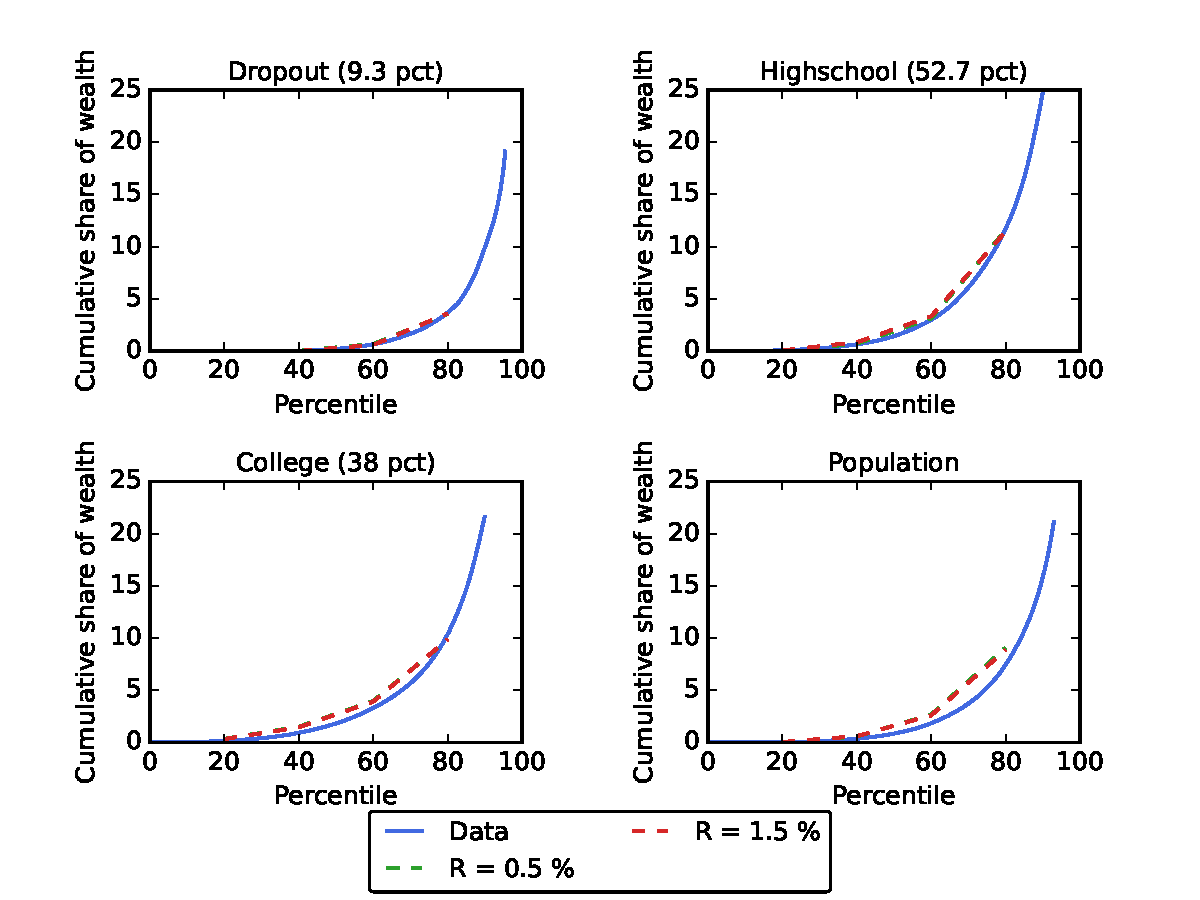
\includegraphics[width=.9\textwidth]{\econtexRoot/Figures/LorenzPoints_robustness_R.pdf}
    \caption{Distributions of liquid wealth within each educational group and for the whole population from the 2004 Survey of Consumer Finance and from the estimated model for different values of the interest rate, $R$.}
    \notinsubfile{\label{fig:LorenzPtsrobustnessR}}
  \end{center}
\end{figure}

\ifthenelse{\boolean{Web}}{}{
\end{document} \endinput
}

